% !TEX options=--shell-escape
\documentclass{beamer}   	% use "amsart" instead of "article" for AMSLaTeX format
\usepackage{geometry}                		% See geometry.pdf to learn the layout options. There are lots.
%\geometry{landscape}                		% Activate for rotated page geometry
%\usepackage[parfill]{parskip}    		% Activate to begin paragraphs with an empty line rather than an indent
\usepackage{graphicx}				% Use pdf, png, jpg, or eps§ with pdflatex; use eps in DVI mode
								% TeX will automatically convert eps --> pdf in pdflatex	

\usepackage{amssymb}
\usepackage{diagbox}
\usepackage{amsmath}
\usepackage{amsthm}
\usepackage{enumerate}
\usepackage{mathrsfs}
\usepackage[utf8]{inputenc}
\usepackage{tikz}
\usepackage[outputdir=build]{minted}
\theoremstyle{definition}
\newtheorem*{defn}{Definition}
\newtheorem*{prop}{Proposition}
\newtheorem*{eg}{Example}
\newtheorem*{thm}{Theorem}
\newtheorem*{corol}{Corollary}
\newtheorem{ex}{Exercise}[section]
{\theoremstyle{plain}
\newtheorem*{rmk}{Remark}
\newtheorem*{rmks}{Remarks}
\newtheorem*{lt}{Last time}
}
\newtheorem*{lem}{Lemma}
\usepackage{color}
\usepackage{CJK}
\usepackage{tcolorbox}
\usepackage{listings}
\newcommand{\rust}[1]{\mintinline{Rust}{#1}}
\newcommand{\husky}[1]{\mintinline{Rust}{#1}}
\newcommand{\cpp}[1]{\mintinline{cpp}{#1}}
\definecolor{lightblue}{rgb}{0.53, 0.81, 0.98}
\useoutertheme{split}
\usecolortheme{whale}
\useinnertheme{rounded} 
\usecolortheme{orchid}
\setbeamertemplate{blocks}[rounded]
\setbeamertemplate{title page}[default][colsep=-4bp,rounded=true]
\setbeamertemplate{part page}[default][colsep=-4bp,rounded=true]
\setbeamertemplate{navigation symbols}{}
\usecolortheme[RGB={148,75,50}]{structure}
% redefine alert block
\setbeamercolor{block title alerted}{use=structure,fg=white,bg=structure.fg!75!black}
\setbeamercolor{block body alerted}{parent=normal text,use=block title,bg=block title.bg!10!bg}


\AtBeginSection[]{ 
  \begin{frame}
  \vfill
  \centering
  \begin{beamercolorbox}[sep=8pt,center,shadow=true,rounded=true]{title}
    \usebeamerfont{title}\insertsectionhead\par%
  \end{beamercolorbox}
  \vfill
  \end{frame}
}

\title{AI Mathematics}
\author{Xiyu Zhai}
\date{}							% Activate to display a given date or no date

\begin{document}
\maketitle

\begin{frame}
\frametitle{AI vs Human}
\begin{itemize}
	\item Physically, AI can be much more energy-consuming than humans, who have evolved for billions of years;
	\item Economically, AI easily beats humans;
	\item Conclusion, AI is meant to replace humans in terms of economic cost.
\end{itemize}
\end{frame}

\begin{frame}
\frametitle{AIGC Takeaway}
\begin{itemize}
	\item Input being natural language, output can be anything;
	\item dramatically lower the threshold to do creative things
	\item empower people's creativity
	\item can this be done for math?
\end{itemize}
\end{frame}

\begin{frame}
\frametitle{AIGC Mathematics}
\begin{itemize}
	\item Applications:
		\begin{itemize}
			\item Education: College Grading, AI tutor, ...
			\item Paper Review
			\item Discovery of new mathematical fact.
		\end{itemize}
	\item Status Quo: LLM can generate natural language math proofs to some limited extent, cannot verify correctness, hallucination.

	One can use LLM to generate formal math proofs to totally avoid hallucination, however the success rate is not high and it's slow. There's a challenge of data.
	\item Reasonable Goal to be Achieved in a Few Years:
	\begin{itemize}
		\item Solve all trivial mathematics. (In a sense, trivial mathematics can be defined to be those solved quickly by AI)
		\item Imitate existing nontrivial proofs.
		\item Search for certain proven theorems and facts.
	\end{itemize}
\end{itemize}
\end{frame}

\begin{frame}
\frametitle{Lack of Formal Mathematics Data}
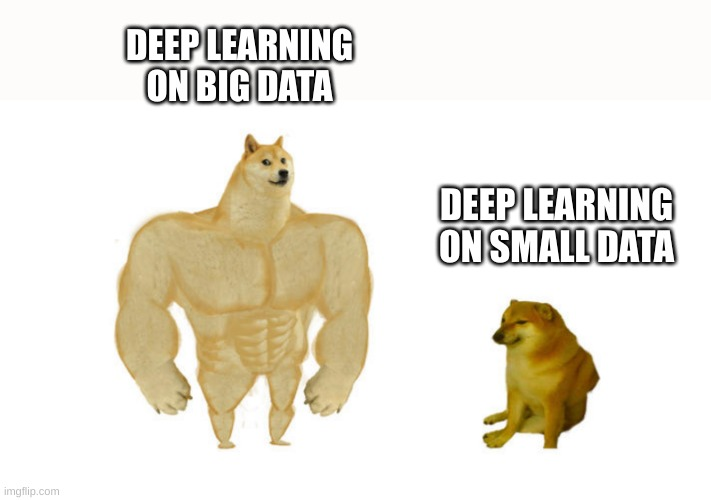
\includegraphics[width=\linewidth]{images/dl_data.jpg}
\end{frame}

\begin{frame}
\frametitle{Existing Mathematics Data is Mostly Natural Language}
\begin{center}
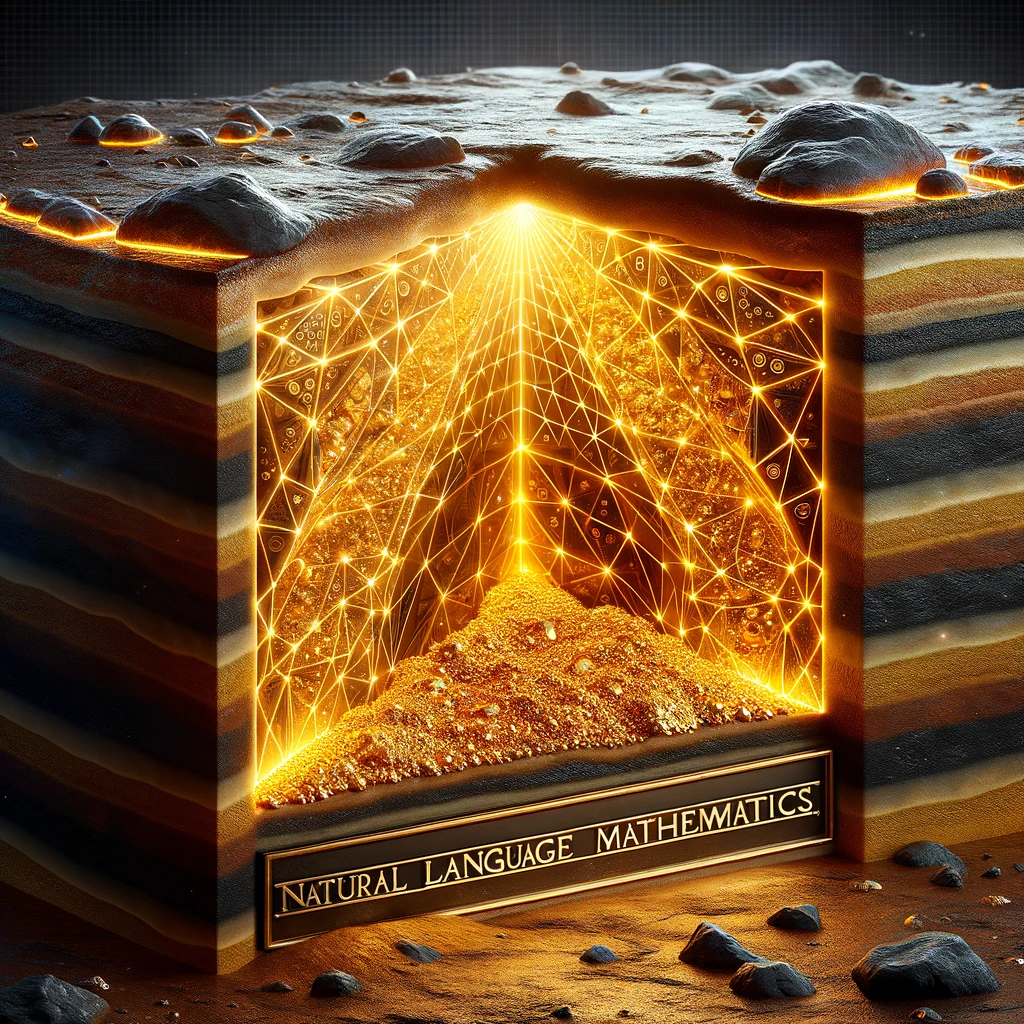
\includegraphics[width=0.7\linewidth]{images/math_gold_mine.png}
\end{center}
\end{frame}

\begin{frame}
\frametitle{The Pain of Formal Verification}
\begin{itemize}
	\item Steep learning curve.
	\item Library. Need to remember the name of the implementation of every tiny facts. Changing all the time.
	\item Small community. Small market. Engineering effort of tooling is poor. Few people mastering.
	\item Formal Verification for Mathematics needs people familiar with both fields, very rare
\end{itemize}
\end{frame}

\begin{frame}
\frametitle{Proof Irrelevance}
\begin{itemize}
	\item 
\end{itemize}
\end{frame}

\end{document}